\subsection{Position, Velocity, Acceleration, Take 2}
Here we have some particular terms we wish to define to carefully define our generalization of the idea of the derivative as the \textit{slope of the tangent line}. Definition vomit ahoy!

\begin{definition}{Position}
If we imagine our parametric curve represents an object's motion in space, then the \textbf{position} function is just the parametric curve $\vcr(t)$ where $$ \vcr(t)=\bmat{x(t)\\y(t)\\z(t)}$$ for some functions $x(t)$, $y(t)$, $z(t)$.
\end{definition}

\begin{definition}{Velocity}
Then velocity, $\vcv(t)$ is just the derivative of position with respect to time. That is, $\vcv(t)=\vcr\hspace{0.2em}'(t)$ or $$\vcv(t)=\bmat{x'(t)\\y'(t)\\z'(t)}.$$
\end{definition}

\begin{definition}{Speed}
You may have heard the phrase ``velocity is a vector and speed is a scalar". Speed is just the scalar version of velocity-- where velocity has a direction, speed is just the magnitue of the velocity vector. That is, $v=||\vcv(t)||=||\vcr\hspace{0.2em}'(t)||.$
\end{definition}

\begin{definition}{Acceleration}
Acceleration is the derivative of velocity with respect to time. That is, $\vca(t)=\vcv\vprime(t)=\vcr\vprime'(t)$.
\end{definition}

Rather than just a slope, however, in order to describe the direction of a function at a given point we need a \textbf{tangent vector}. We also generally wish to just describe the \textit{direction} of the change of the function rather than the \textit{magnitude} of the change. Because of this, we desire that our tangent vector be a unit vector. So then we get the following definition.

\begin{definition}{Tangent Vector}
The \textbf{tangent vector} for a function, $\vcT(t)$ is the unit vector parallel to the velocity vector. That is, $$\vcT(t)=\frac{\vcv(t)}{v}=\frac{\vcv(t)}{||\vcv(t)||}=\frac{\vcr\vprime(t)}{||\vcr\vprime{t}||}. $$
\end{definition}

Note that this yields the equation of a tangent line in 3-d.

\begin{definition}{Tangent Line}
Let $\vcr(t)$ be a vector function in $n$-dimensional space and let $\vcv(t)$ be the $\vcr\vprime(t)$. Then the equation of the line tangent to $\vcr(t)$ at $t=a$ in parametric form is $$\vcl(t)=\vcv(a)\cdot t+\vcr(a). $$
\end{definition}

We get a couple of followup definitions out of this. In particular, since these functions are often changing directions, we get an idea of \textbf{angular velocity}.

\begin{definition}{Angular Velocity}
The \textbf{angular velocity} for a function $\vcr(t)$ is the change in the tangent vector. That is, $$\vomega(t)=\vcT\vprime(t). $$
\end{definition}

\begin{definition}{Angular Speed}
Just like velocity to speed, angular speed is just the magnitude of angular velocity. That is, $$\omega(t)=||\vomega(t)||=||\vcT\vprime(t)||. $$
\end{definition}

This angular velocity idea lets us define the \textbf{normal vector} for a function. Where the tangent vector indicates the direction of motion of the function, the normal vector indicates the direction of change for the \textit{tangent vector itself}.

\begin{definition}{Normal Vector}
The \textbf{normal vector} to a function $\vcr(t)$ is the unit vector parallel to the angular velocity. That is, $$\vcN(t)=\frac{\vomega(t)}{\omega(t)}=\frac{\vcT\vprime(t)}{||\vcT\vprime(t)||}. $$
\end{definition}

\begin{example}{Tangents and Normals}
Let's consider the position function $$\vcr(t)=\bmat{\sin(t)\\ \cos(t)\\t}. $$
This generates a helix.
\begin{center}
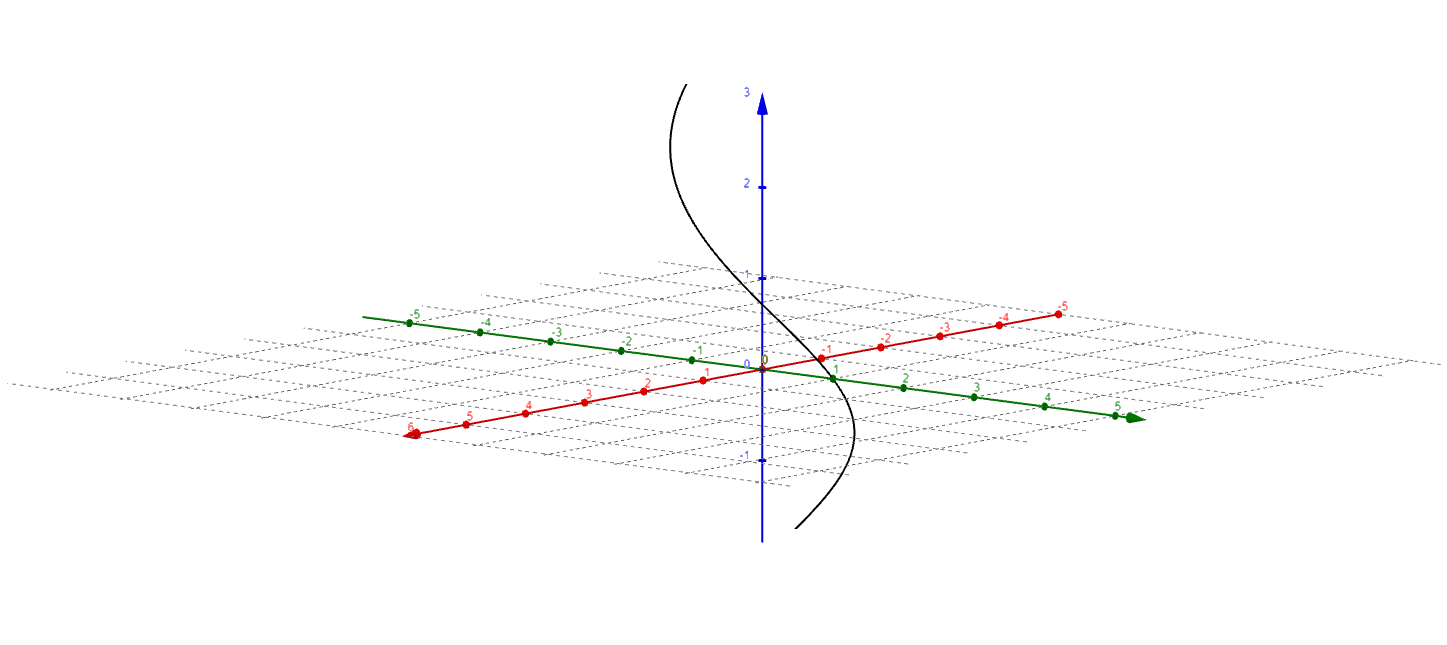
\includegraphics[scale=0.3]{Figures/tangentnormalex}
\\
Graph of $\vcr(t)$.
\end{center}
\vspace{1em}
Finding the velocity of object is a matter of taking the derivative component-wise:
$$\vcv(t)=\bmat{\cos(t)\\-\sin(t)\\1}. $$
Then we can find $v$, the speed:
\begin{align*}
v=&||\vcv||\\
=&\sqrt{\cos^2(t)+(-\sin(t))^2+1^2}\\
=&\sqrt{\cos^2(t)+\sin^2(t)+1}\\
=&\sqrt{2}.
\end{align*}
Then we can find the tangent vector $$\vcT(t)=\frac{\vcv}{v}=\bmat{\frac{\cos t}{\sqrt2}\\ -\frac{\sin t}{\sqrt2}\\ \frac{1}{\sqrt{2}}}.$$
From there, to find the normal vector we differentiate for the angular velocity, then normalize.
$$\vomega(t)=\vcT\vprime(t)=\bmat{\frac{-\sin t}{\sqrt{2}}\\ \frac{-\cos t}{\sqrt{2}}\\ 0}.$$
The angular speed, $||\vcT\vprime(t)||=\frac{1}{\sqrt{2}}$, so our normal vector is $$\vcN(t)=\frac{\vomega}{\omega}=\bmat{-\sin t\\ -\cos t\\ 0}. $$
You can visit this \href{https://www.geogebra.org/3d/rfrp5b9b}{Geogebra link} to view the function, along with it's tangent and normal vector (tangent in blue, normal in red). You can vary the value of $a$ to move the tangent/normal vectors along the curve and see how they change along the path.
\end{example}

\begin{exercise}{Tangents and Normals}\label{tandn}
Let $$\vcr(t)=\bmat{t\\2\sin(t)\\2\cos(t)} .$$
\begin{enumerate}
\item Find the tangent vector $\vcT(t)$.
\vspace{1em}
\item Find the equation of the line tangent $\vcr(t)$ at $t=\frac{\pi}{3}$ in parametric form. (your direction vector can just be the velocity vector to the function at the given point!) \href{https://www.geogebra.org/3d/cngzwkaw}{Geogebra Link}
\vspace{1em}
\item Find the normal vector $\vcN(t)$.
\vspace{1em}
\item Of occasional use is the \textbf{binormal vector}, which is the cross product of the tangent and normal vectors. Compute the binormal vector for $r(t)$.
\end{enumerate}
\end{exercise}